\startchapter{Hardware Trojans}
\label{chapter:hardwareTrojans}

\newlength{\savedunitlength}
\setlength{\unitlength}{2em}
\section{Background} \label{sec:trojanBackGround}
\acrfull{ICs} are continuously decreasing in size whilst increasing in complexity.
These trends require ever more people and sophisticated means of manufacture which in turn creates security vulnerabilities.
Products developed by semiconductor companies generally compromised in one of two ways.
First, due to the complexity it is rare for a product to be managed within a single company.
Frequently, steps in the production-chain are outsourced.
It is within these 'third-party' contributors that products can be maliciously modified.
Secondly, for various reasons, employees of trusted contributors have been known to make modifications.~\cite{trojanSurvey2014}
These modifications are known as hardware Trojans.
\acrshort{IC}s are an integral part of every facet of the modern world.
Proper application of a Trojan can provide information, control of mechanical systems, surveillance and more to an unauthorized party.
\section{Topology} \label{sec:topology}
The discussion, detection and evaluation of hardware trojans requires a comprehensive means of description.
Several hardware trojan taxonomies have been proposed~\cite{taxonomy1, taxonomy2, taxonomy3, taxonomy4}.
In~\cite{taxonomy1}, trojans were organized based solely on their activation mechanisms.
A taxonomy based on the location, activation and action of a trojan was presented in \cite{taxonomy2}, \cite{taxonomy3}.
However, these approaches do not consider the manufacturing process.
Another taxonomy was proposed in~\cite{taxonomy4} which employs five categories: insertion, abstraction, activation, effect, and location.
While this is more extensive than previous approaches, it fails to account for the physical characteristics of a trojan.
An additional taxonomy was proposed in~\cite{samerAttribute} which considers all attributes a hardware trojan may posses.
This taxonomy is the most comprehensive and was selected as the means of description for this work.
\begin{figure}
	\centering
	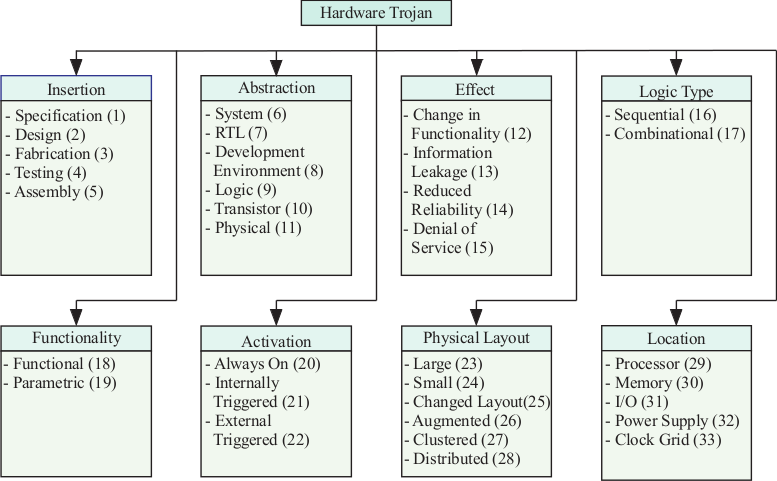
\includegraphics[width=1.0\linewidth]{figures/HW_trojan}
	\caption{The thirty-three attributes of the hardware trojan taxonomy in~\cite{samerAttribute}.}
	\label{fig:HW_trojan}
\end{figure}
It is comprised of thirty-three attributes organized into eight categories as shown in Fig.~\ref{fig:HW_trojan}.
These categories can be arranged into the following four levels as indicated in Fig.~\ref{fig:trojan_life_cycle}.
\begin{enumerate}
	\item The \textbf{insertion} (chip life-cycle) level/category comprises the attributes pertaining to the IC production stages.
	\item The \textbf{abstraction} level/category corresponds to where in the IC abstraction the trojan is introduced.
	\item The \textbf{properties} level comprises the behavior and physical characteristics of the trojan.
	\item The \textbf{location} level/category corresponds to the location of the trojan in the IC.
\end{enumerate}
The properties level consists of the following categories.
\begin{itemize}
	\item The \textbf{effect} describes the disruption or effect a trojan has on the system.
	\item The \textbf{logic type} is the circuit logic that triggers the trojan, either combinational or sequential.
	\item The \textbf{functionality} differentiates between trojans which are functional or parametric.
	\item The \textbf{activation} differentiates between trojans which are always on or triggered.
	\item The \textbf{layout} is based on the physical characteristics of the trojan.
\end{itemize}
\begin{figure}
	\centering
	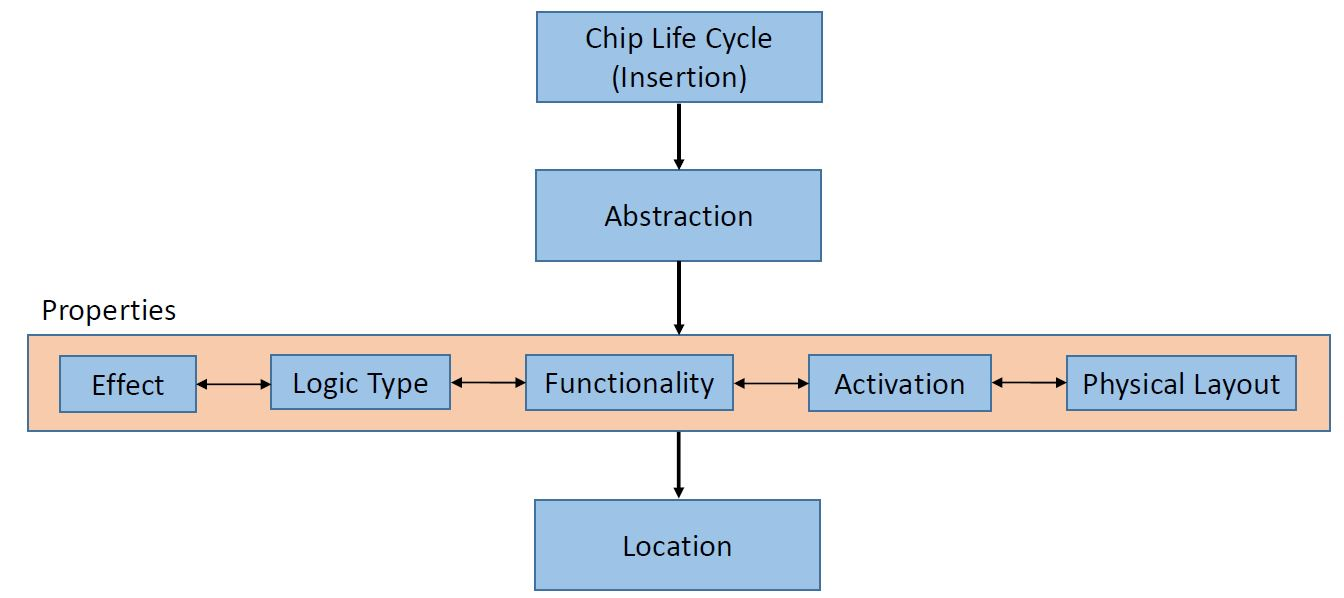
\includegraphics[width=0.8\linewidth]{figures/trojan_life_cycle}
	\caption{The hardware trojan levels \cite{samerAttribute}.}
	\label{fig:trojan_life_cycle}
\end{figure}

\begin{table*}
	\[
	\newcommand\scalemath[2]{\scalebox{#1}{\mbox{\ensuremath{\displaystyle #2}}}}
	\mathbf{R} =
	\left[
	\scalemath{0.5}{
		\begin{array}{l||c|c|c|c|c||c|c|c|c|c|c||c|c|c|c|c|c|c|c|c|c|c|c|c|c|c|c|c||c|c|c|c|c}
		A & 1$~$ & 2$~$  & 3$~$ & 4$~$& 5$~$ & 6$~$  & 7$~$ & 8$~$ & 9$~$ & 10  & 11 & 12& 13 & 14  & 15 & 16& 17 & 18  & 19 & 20& 21 & 22  & 23 & 24& 25 & 26  & 27 & 28 & 29 &30 & 31 & 32 & 33\\ \hline \hline
		1 & 0 & 1 & 0 & 0 & 0 & 1 & 0 & 0 & 0 & 0 & 0 &  &  &  &  &  &  &  &  &  &  &  &  &  &  &  &  &   &  &  &  &  &  \\ \hline
		2 & 0 & 0 & 1 & 0 & 0 & 0 & 1 & 0 & 0 & 0 & 0 &  &  &  &  &  &  &  &  &  &  &  &  &  &  &  &  & &  &  &  &  &   \\ \hline
		3 & 0 & 0 & 0 & 1 & 0 & 0 & 0 & 0 & 0 & 0 & 1 &  &  &  &  &  &  &  &  &  &  &  &  &  &  &  &  & &  &  &  &  &   \\  \hline
		4 & 0 & 0 & 0 & 0 & 1 & 1 & 0 & 0 & 1 & 0 & 0 &  &  &  &  &  &  &  &  &  &  &  &  &  &  &  &  &&  &  &  &  &    \\  \hline
		5 & 0 & 0 & 0 & 0 & 0 & 1 & 0 & 0 & 0 & 0 & 0 &  &  &  &  &  &  &  &  &  &  &  &  &  &  &  &  &  &  &  &  &  &  \\  \hline \hline
		6 &  &  &  &  &  & 0 & 1 & 0 & 0 & 0 & 0 &1 & 1 & 0 & 1 & 0 & 0 & 1 & 1 & 1 & 0 & 0 & 0 & 0 & 0 & 0 & 0 & 0  &  &  &  &  &  \\ \hline
		7 &  &  &  &  &  & 0 & 0 & 1 & 0 & 0 & 0 &1 & 0 & 0 & 1 & 1 & 1 & 1 & 0 & 1 & 1 & 1 & 1 & 1 & 0 & 0 & 0 & 0  &  &  &  &  &   \\ \hline
		8 &  &  &  &  &  & 0 & 0 & 0 & 1 & 0 & 0 &1 & 0 & 0 & 1 & 1 & 1 & 1 & 0 & 1 & 1 & 1 & 1 & 1 & 1 & 1 & 1 & 1  &  &  &  &  &   \\ \hline
		9 &  &  &  &  &  & 0 & 0 & 0 & 0 & 1 & 0 & 1 & 0 & 0 & 1 & 1 & 1 & 1 & 0 & 1 & 1 & 1 & 0 & 0 & 0 & 0 & 0 & 0 &  &  &  &  &    \\ \hline
		10 &  &  &  &  &  & 0 & 0 & 0 & 0 & 0 & 1 & 1 & 0 & 1 & 0 & 0 & 1 & 1 & 1 & 1 & 0 & 0 & 0 & 1 & 0 & 1 & 1 & 0  &  &  &  &  &  \\  \hline
		11 &  &  &  &  &  & 0 & 0 & 0 & 0 & 0 & 0 &1 & 1 & 1 & 0 & 0 & 0 & 1 & 1 & 1 & 0 & 0 & 1 & 1 & 1 & 1 & 1 & 1  &  &  &  &  &    \\  \hline \hline
		12 & &  &  &  &  &  &  &  &  &  &  & 0 & 0 & 0 & 0 & 1 & 1 & 1 & 0 & 1 & 1 & 1 & 1 & 1 & 1 & 1 & 1 & 1&1 & 1 & 1 & 1 & 1 \\ \hline
		13 & &  &  &  &  &  &  &  &  &  &  &0 & 0 & 0 & 0 & 0 & 1 & 0 & 1 & 1 & 0 & 1 & 0 & 1 & 0 & 1 & 1 & 1&1 & 1 & 1 & 1 & 1 \\ \hline
		14 &&  &  &  &  &  &  &  &  &  &  & 0 & 0 & 0 & 0 & 0 & 0 & 0 & 1 & 1 & 0 & 0 & 0 & 1 & 0 & 1 & 1 & 1&1 & 1 & 1 & 1 & 1 \\ \hline
		15 & &  &  &  &  &  &  &  &  &  &  &0 & 0 & 0 & 0 & 1 & 1 & 1 & 0 & 1 & 1 & 1 & 1 & 1 & 1 & 1 & 1 & 1&1 & 0 & 1 & 1 & 1 \\ \hline
		16 & &  &  &  &  &  &  &  &  &  &  &1 & 0 & 0 & 1 & 0 & 0 & 1 & 0 & 0 & 1 & 1 & 1 & 0 & 1 & 1 & 1 & 1&1 & 1 & 1 & 1 & 1 \\ \hline
		17 & &  &  &  &  &  &  &  &  &  &  &1 & 1 & 0 & 1 & 0 &0 & 1 & 0 & 1 & 1 & 1 & 1 & 1 & 1 & 1 & 1 & 1&1 & 1 & 1 & 1 & 1 \\ \hline
		18 & &  &  &  &  &  &  &  &  &  &  &1 & 0 & 0 & 1 & 1 & 1 & 0 & 0 & 1 & 1 & 1 & 1 & 1 & 1 & 1 & 1 & 1&1 & 1 & 1 & 1 & 1 \\ \hline
		19 & &  &  &  &  &  &  &  &  &  &  &0 & 1 & 1 & 0 & 0 & 0 & 0 & 0 & 1 & 0 & 0 & 0 & 1 & 0 & 1 & 0 & 1&0 & 0 & 1 & 1 & 1 \\ \hline
		20 & &  &  &  &  &  &  &  &  &  &  &1 & 1 & 1 & 1 & 0 & 1 & 1 & 1 & 0 & 0 & 0 & 1 & 1 & 1 & 1 & 1 & 1&1 & 1 & 1 & 1 & 1 \\ \hline
		21 & &  &  &  &  &  &  &  &  &  &  &1 & 0 & 0 & 1 & 1 & 1 & 1 & 0 & 0 & 0 & 0 & 1 & 1 & 0 & 1 & 1 & 1&1 & 1 & 1 & 1 & 1 \\ \hline
		22 & &  &  &  &  &  &  &  &  &  &  &1 & 1 & 0 & 1 & 1 & 1 & 1 & 0 & 0 & 0 & 0 & 0 & 1 & 0 & 1 & 1 & 0&1 & 1 & 1 & 1 & 1 \\ \hline
		23 & &  &  &  &  &  &  &  &  &  &  &1 & 0 & 0 & 1 & 1 & 1 & 1 & 0 & 1 & 1 & 0 & 0 & 0 & 1 & 1 & 1 & 1&1 & 1 & 0 & 0 & 0  \\ \hline
		24 & &  &  &  &  &  &  &  &  &  &  &1 & 1 & 1 & 1 & 0 & 1 & 1 & 1 & 1 & 1 & 1 & 0 & 0 & 0 & 1 & 1 & 0&1 & 1 & 1 & 1 & 1 \\ \hline
		25 &&  &  &  &  &  &  &  &  &  &  & 1 & 0 & 0 & 1 & 1 & 1 & 1 & 0 & 1 & 0 & 0 & 1 & 0 & 0 & 1 & 1 & 0& 1 & 1 & 1 & 1 & 1\\ \hline
		26 & &  &  &  &  &  &  &  &  &  &  &1 & 1 & 1 & 1 & 1 & 1 & 1 & 1 & 1 & 1 & 1 & 1 & 1 & 1 & 0 & 1 & 1& 1 & 1 & 1 & 1 & 1\\ \hline
		27 & &  &  &  &  &  &  &  &  &  &  &1 & 1 & 1 & 1 & 1 & 1 & 1 & 0 & 1 & 1 & 1 & 1 & 1 & 1 & 1 & 0 & 0 &1 & 1 & 1 & 1 & 1\\ \hline
		28 & &  &  &  &  &  &  &  &  &  &  &1 & 1 & 1 & 1 & 1 & 1 & 1 & 1 & 1 & 1 & 0 & 1 & 0 & 0 & 1 & 0 &0 &1 & 1 & 1 & 1 & 1\\ \hline \hline
		29 & &  &  &  &  &  &  &  &  &  &  & &  &  & &  &  &  &  &  &  &  &  &  &  &  &  & & &  &  &  & \\ \hline
		30 & &  &  &  &  &  &  &  &  &  &  & &  &  & &  &  &  &  &  &  &  &  &  &  &  &  & & &  &  &  & \\ \hline
		31 & &  &  &  &  &  &  &  &  &  &  & &  &  & &  &  &  &  &  &  &  &  &  &  &  &  & & &  &  &  & \\ \hline
		32 & &  &  &  &  &  &  &  &  &  &  & &  &  & &  &  &  &  &  &  &  &  &  &  &  &  & & &  &  &  & \\ \hline
		33 & &  &  &  &  &  &  &  &  &  &  & &  &  & &  &  &  &  &  &  &  &  &  &  &  &  & & &  &  &  & \\
		\end{array}
	}
	\right ]
	\label{ss1}
	\]
\end{table*}
The relationships between the trojan attributes shown in Fig.~\ref{fig:HW_trojan} can be described using a matrix $\mathbf{R}$~\cite{samerAttribute}.
%Systematic analysis of matrix $\mathbf{R}$ provides useful insight into the overall nature of a subject.
%A procedure used to develop the nature of a subject has been described in~\cite{samerAttribute} and is referred to as Classification.
Entry $r(i,j)$ in $\mathbf{R}$ indicates whether or not attribute $i$ can lead to attribute $j$.
For example, $r(2,3) = 1$ indicates that design (attribute 2) can lead to fabrication (attribute 3).
This implies that if an IC can be compromised during the design phase (attribute 2), it may influence the fabrication phase (attribute 3).

The matrix $\mathbf{R}$ is divided into sub matrices as follows
\[
\newcommand\scalemath[2]{\scalebox{#1}{\mbox{\ensuremath{\displaystyle #2}}}}
\mathbf{R} =\left[
\scalemath{1.1}{
	\begin{array}{l*{3}{c}}
	\mathbf{R_1} ~ & ~ \mathbf{R_{12}} ~ & ~ 0 ~  &  ~ 0   \\
	0         & \mathbf{R_2}      &\mathbf{R_{23}}       & ~ 0 \\
	0          & 0           & \mathbf{R_3}          & ~ \mathbf{R_{34}} \\
	0          & 0           & 0                & ~ \mathbf{R_4} \\
	\end{array}
}
\right]
\label{R}
\]
where $\mathbf{R_1}$, $\mathbf{R_2}$, $\mathbf{R_3}$ and $\mathbf{R_4}$ indicate the attribute relationships within a category.
For example, $\mathbf{R_1}$ is given by
\[
\newcommand\scalemath[2]{\scalebox{#1}{\mbox{\ensuremath{\displaystyle #2}}}}
\mathbf{R_1} =\left[
\scalemath{1.0}{
	\begin{array}{l|*{11}{c}}
	A & 1$~$ & 2$~$  & 3$~$ & 4$~$& 5$~$\\ \hline
	1 & 0 & 1 & 0 & 0 & 0  \\
	2 & 0 & 0 & 1 & 0 & 0  \\
	3 & 0 & 0 & 0 & 1 & 0  \\
	4 & 0 & 0 & 0 & 0 & 1  \\
	5 & 0 & 0 & 0 & 0 & 0  \\
	\end{array}
}
\right ]
\label{R1}
\]
Submatrix $\mathbf{R_{12}}$ relates the attributes of the insertion category to the attributes of the abstraction category.
An example of this submatrix is
\[
\newcommand\scalemath[2]{\scalebox{#1}{\mbox{\ensuremath{\displaystyle #2}}}}
\mathbf{R_{12}} =\left[
\scalemath{1.0}{
	\begin{array}{l|*{11}{c}}
	A & 6$~$  & 7$~$ & 8$~$ & 9$~$ & 10  & 11\\ \hline
	1  & 1 & 0 & 0 & 0 & 0 & 0 \\
	2  & 0 & 1 & 0 & 0 & 0 & 0 \\
	3  & 0 & 0 & 0 & 0 & 0 & 1 \\
	4  & 1 & 0 & 0 & 1 & 0 & 0 \\
	5  & 1 & 0 & 0 & 0 & 0 & 0 \\
	\end{array}
}
\right ]
\label{R12}
\]

\section{\acrfull{FPGAs}}
An \acrshort{IC} belongs to one of two categories.
An \acrfull{ASIC} or a \acrfull{FPGA}.
An \acrshort{ASIC} is manufactured once and is immutable; its hardware is permanently printed in silicon.
\acrshort{FPGA}s are reconfigurable.
They are comprised of an array of \acrfull{PLDs}.
A \acrshort{PLD} is a component whose functionality is dependent on a set of configuration options.
Each \acrshort{PLD} in and \acrshort{FPGA} device receives a series of configuration instructions in the form of a binary message.
A single \acrshort{FPGA} can contain hundreds, or even thousands of \acrshort{PLD}s, each of which can be one of hundreds of possible different types.
The messages from all \acrshort{PLD}s comprise the configuration \gls{Bitstream} for the whole device. 
\acrshort{FPGA} developers create processor designs using a programming language; the design is then downloaded or "configured" onto the device via the \gls{Bitstream}.
The design process is simpler and modifications can be made after manufacture.
Because of this, \acrshort{FPGA}s are becoming the \acrshort{IC} of choice in larger scale productions however these same features increase their vulnerability.


\setlength{\unitlength}{\savedunitlength}